% % % % % % % % % % % % % % % % % % % % % % % % % % % % % % % % % % % % % % % % % % % %
%                                                                                     %
% Short Sectioned Assignment LaTeX Template Version 1.0 (5/5/12)                      %
% This template has been downloaded from: http://www.LaTeXTemplates.com               %
%                                                                                     %
% Original author:  Frits Wenneker (http://www.howtotex.com)                          %
%                                                                                     %
% Modified by: Fco Javier Sueza Rodríguez (fcosueza@disroot.org)                      %
%                                                                                     %
% Changes:                                                                            %
%	    - Custom Chapters, Sections and Subsections (titlesec package)                %
%           - Document type scrbook (oneside)                                         %
%           - Use babel-lang-spanish package and marvosym                             %
%           - Use hyperref, enumitem, tcolorbox and glossaries packages               %
%           - Use Time New Roman (mathptmx), Helvetic and Courier fonts               %
%                                                                                     %
% License: CC BY-NC-SA 3.0 (http://creativecommons.org/licenses/by-nc-sa/3.0/)        %
%                                                                                     %
% % % % % % % % % % % % % % % % % % % % % % % % % % % % % % % % % % % % % % % % % % % %

%-----------------------------------------------%
%	              Packages                  %
%-----------------------------------------------%

\documentclass[paper=a4, fontsize=11pt, oneside]{scrbook}

% ---- Text Input/Output ----- %

\usepackage[T1]{fontenc}
\usepackage[utf8]{inputenc}
\usepackage{mathptmx}
\usepackage[scaled=.92]{helvet}
\usepackage{courier}
\usepackage[indent=12pt]{parskip}

\usepackage{geometry}
\geometry{verbose,tmargin=3cm,bmargin=3cm,lmargin=2.6cm,rmargin=2.6cm}

% ---- Language ----- %

\usepackage[spanish]{babel}
\usepackage{marvosym}

% ---- Another packages ---- %

\usepackage{amsmath,amsfonts,amsthm}
\usepackage{graphics,graphicx}
\usepackage{titlesec}
\usepackage{fancyhdr}
\usepackage{tcolorbox}
\usepackage{hyperref}
\usepackage{enumitem}
\usepackage[automake]{glossaries}

%--------------------------------------------------------------------%
%                      Customizing Document                          %
%--------------------------------------------------------------------%


% ----------- Custom Chapters, Sections and Subsections -------------- %

\titleformat{\chapter}[display]
			{\bfseries\Huge}
			{Tema \ \thechapter} {0.5ex}
			{\vspace{1ex}\centering}

\titleformat{\section}[hang]
			{\bfseries\Large}
			{\thesection}{0.5em}{}

\titleformat{\subsection}[hang]
			{\bfseries\large}
			{\thesubsection}{0.5em}{}

\titleformat{\subsubsection}[hang]
			{\bfseries\large}
			{\thesubsubsection}{0.5em}{}

\hypersetup{
    colorlinks=true,
    linkcolor=black,
    urlcolor=magenta
}

% ------------------- Custom heaaders and footers ------------------- %

\pagestyle{fancyplain}

\fancyhead[]{}
\fancyfoot[L]{}
\fancyfoot[C]{}
\fancyfoot[R]{\thepage}

\renewcommand{\headrulewidth}{0pt} % Remove header underlines
\renewcommand{\footrulewidth}{0pt} % Remove footer underlines

\setlength{\headheight}{13.6pt} % Customize the height of the header

% --------- Numbering equations, figures and tables ----------------- %

\numberwithin{equation}{section} % Number equations within sections
\numberwithin{figure}{section} % Number figures within sections
\numberwithin{table}{section} % Number tables within sections

% ------------------------ New Commands ----------------------------- %

\newcommand{\horrule}[1]{\rule{\linewidth}{#1}} % Create horizontal rule command


%----------------------------------------------------------------------------------------
%	TÍTULO Y DATOS DEL ALUMNO
%----------------------------------------------------------------------------------------

\title{
\normalfont \normalsize
\textsc{{\bfseries Curso 2022-2023} \\ Ciclo Superior de Desarrollo de Aplicaciones Web \\ IES Aguadulce} \\ [25pt]
\horrule{0.5pt} \\[0.4cm]
\huge Sistemas Informáticos \\
\horrule{0.5pt} \\[0.4cm]
}

\author{Francisco Javier Sueza Rodríguez}
\date{\normalsize\today}

%----------------------------------------------------------------------------------------
%                                     DOCUMENTO
%----------------------------------------------------------------------------------------
\makeglossaries
\loadglsentries{glossary.tex}

\begin{document}

\maketitle

\newpage

\tableofcontents

\listoffigures

%\listoftables

\newpage

\chapter{Hardware de un Sistemas Informático}
En esta primera unidad de la asignatura ``\textbf{Sistemas Informáticos}, vamos a ver los conceptos básicos de sobre los sistemas informáticos, centrándonos principalmente en el apartado del hardware de un sistema informático. Así, veremos cuales son los diferentes componente hardware (o físicos) de un computador, así como la información necesaria para su ensamblaje y puesta en marcha.

También veremos diferentes tipos de clasificaciones de los ordenadores, incluyendo los ordenadores personales, así como otra información útil que podremos encontrar en los diferentes anexos que se incluyen al final de esta unidad.

\section{Sistema Informático}
La \textbf{informática} es la ciencia que se encarga de estudiar todo lo relacionado con los sistemas informáticos, incluyendo los temas relativos a su arquitectura y fabricación, hasta los temas referidos al almacenamiento y organización de la información, sin olvidar la creación y uso de software, o la formación del personal informático. Para ello, se apoya en múltiples disciplinas como las matemáticas, física, electrónica, etc...

Un \textbf{sistema informático} es el conjunto de \textbf{elementos físicos} (hardware) y \textbf{elementos lógicos} (software), interconectados entre sí, destinados a gestionar el \textbf{tratamiento automático de la información}, entendiendo por esto, su almacenamiento, transmisión, organización y/o procesamiento.

Se incluye, como parte fundamental de un sistema informático, al \textbf{conjunto de personas} que lo \textbf{utiliza}, ya sean usuario, administradores, programadores, etc... El elemento humano es un \textbf{componente imprescindible}, ya que los sistemas informáticos son creados, desarrollados y utilizados por humanos para su propio provecho.

En sistema informáticos siempre debemos distinguir entre hardware y software:

\begin{itemize}
    \item \textbf{Hardware}: son todos los elementos físicos que forman parte de un ordenador, es decir, teclado, ratón, placa base, monitor, memoria, disco duro, cables, etc... Es la ``maquinaria'' necesaria utilizada para el tratamiento de la información.
    \item \textbf{Software}: es el elemento lógico e ``intangible'' de un sistema informático. Se compone de un conjunto de programas y datos que permiten manejar el hardware, controlando y coordinando su funcionamiento para que pueda realizar las tareas esperadas. Esta compuesto principalmente de dos elementos:
    \begin{itemize}
        \item \textbf{Programas}: están formados por un conjunto de órdenes o instrucciones que se utilizan para procesador los datos que se introducen como información. Son necesarios para la gestión y el control de los equipos y los trabajos de los usuarios.
        \item \textbf{Datos}: son la información que los programas deben procesar, utilizando para esto diferentes elementos hardware que componen el sistema informático. Son, en definitiva, la razón de ser el sistema informático.
    \end{itemize}
\end{itemize}

Los \textbf{sistemas informáticos} han \textbf{evolucionado}. En un principio todos sus componentes, físicos, lógicos y humanos, estaban localizados en el mismo lugar, pero actualmente están formados por subsistemas que se interconectan a través de la red, que pueden llegar a estar a miles de kilómetros de distancia entre sí, integrando sistemas complejos de procesamiento de la información. Estos subsistemas a si vez pueden estar compuestos por un superodenador, un ordenador personal, redes locales de ordenadores o por una combinación de todos ellos, siendo el sistema informático más simple el formado por un ordenador y un usuario que ejecuta programas en él.

Un \textbf{ordenador} se define como una máquina electrónica, con algunas partes mecánicas, compuesta por al menos, una unidad de proceso, y por equipos periféricos, controlada por programas que deben estar almacenados en su memoria central, destinada al tratamiento automático de la información que le es suministrada. Es una máquina de propósito general ya que puede realizar gran variedad de trabajos y a gran velocidad.

En el \textit{Anexo A.1}, podrás encontrar más información sobre la clasificación de los ordenadores.

\section{Arquitectura Hardware: Componentes Funcionales}
Un computador es compuesto por una seria de sistemas y subsistemas hardware, que cooperando entre sí, permiten a este llevar a cabo su función, procesando la información que recibe y emitiendo los resultados de este procesado.  Estos subsistemas consta, principalmente de tres elementos:

\begin{itemize}
    \item \textbf{Unidad Central de Proceso} (CPU): es el sistemas básico más importante, encargado de coordinar a los demás subsistemas, extraer secuencialmente las instrucciones de la memoria principal para procesarlas y ejecutarlas.
    \item \textbf{Sistemas de Memoria}: su función básica es la de almacenar las instrucciones que se van a procesar posteriormente, los datos y los resultados que sean necesarios.
    \item \textbf{Periféricos}: se dividen en periféricos de entrada y de salida, según la dirección del flujo de información. Ambos sistemas se encargan de la comunicación con el exterior, es decir, con el usuario u otros sistemas.
\end{itemize}

Estos subsistemas se interconectan mediante un \textbf{bus de sistema}, que consta de un conjunto de conexiones físicas encargado de transmitir la información entre los diferentes subsistemas. En la siguiente figura, podemos ver un esquema de esta arquitectura.

\begin{figure}[ht]
    \centering
    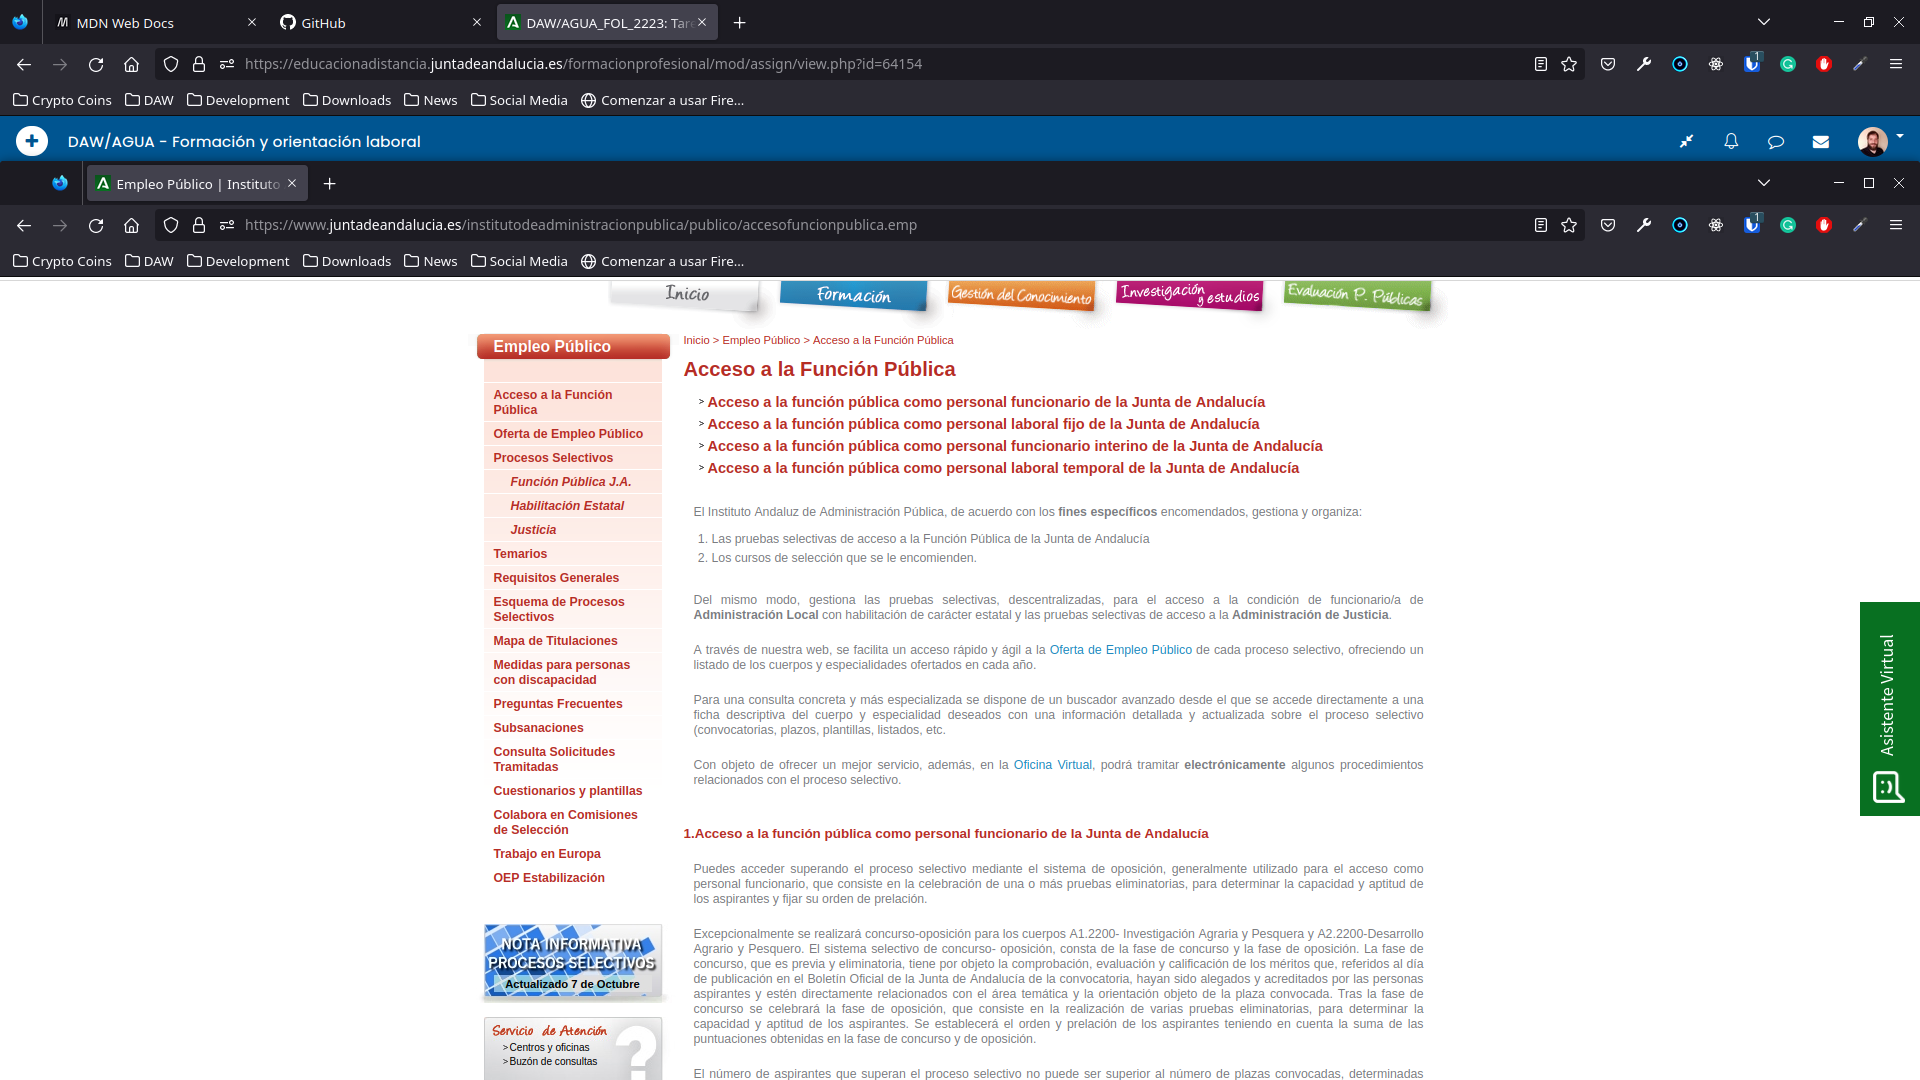
\includegraphics[scale=0.25]{empleo-iaap.png}
    \caption{Subsistemas de un Computador}
\end{figure}

% Glossary

\glsaddall
\printglossaries

% Bibliography

\newpage
\addcontentsline{toc}{chapter}{Bibliografía}
\bibliography{citas}
\bibliographystyle{unsrt}

\end{document}